\begin{tiny}(Ega04)\end{tiny}
Dans cet exercice, on utilise les conditions d'alignement ou de concours de l'exercice ga01 et des calculs de déterminants des exercices dt25 et dt26. 
\begin{figure}[h!]
  \centering
  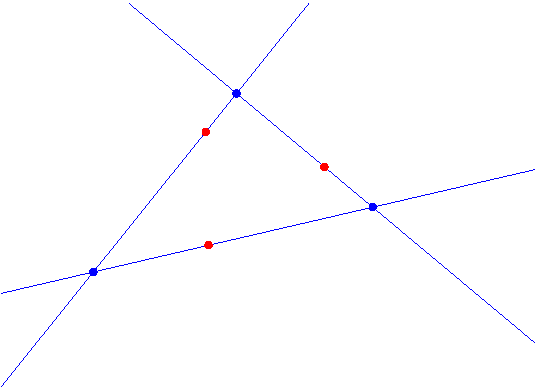
\includegraphics[width=7cm]{Ega04_1.pdf}
  % Egp11_1.pdf: 170x107 px, 72dpi, 6.00x3.77 cm, bb=0 0 170 107
  \caption{Exercice \arabic{enumi} a.: théorème de Ménéla{\"u}s.}
  \label{fig:Ega04_1}
\end{figure}

\begin{figure}[h!]
  \centering
  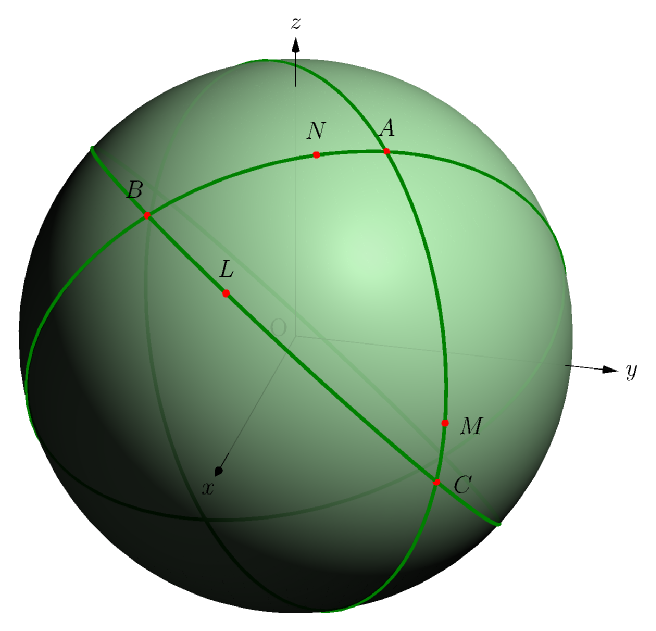
\includegraphics[width=7cm]{Ega04_2.eps}
  % Ega04_2.eps: 1229x1345 px, 300dpi, 10.41x11.39 cm, bb=158 234 453 557
  \caption{Exercice \arabic{enumi} c.: Ménéla{\"u}s en géométrie sphérique.}
  \label{fig:Ega04_2}
\end{figure}

\begin{figure}[h!]
  \centering
  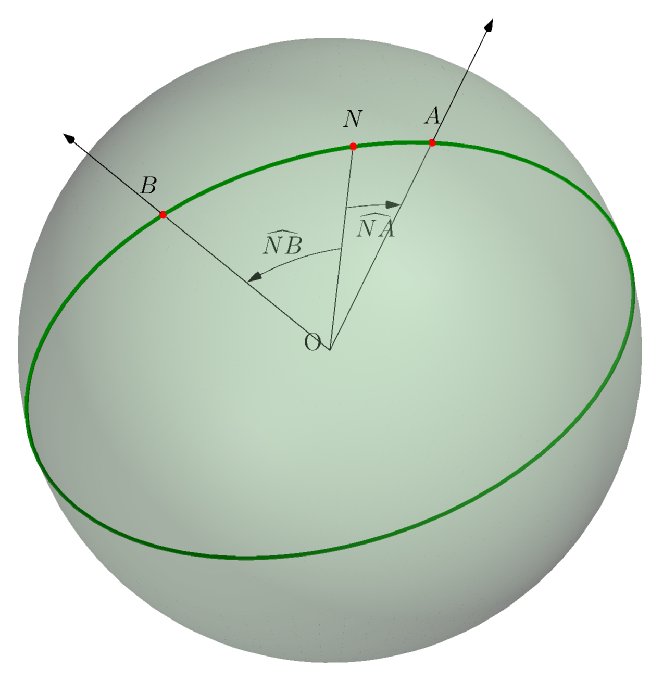
\includegraphics[width=7cm]{Ega04_3.eps}
  % Ega04_2.eps: 1229x1345 px, 300dpi, 10.41x11.39 cm, bb=158 234 453 557
  \caption{Exercice \arabic{enumi} c.: Repérage sur un grand cercle.}
  \label{fig:Ega04_3}
\end{figure}

Les points $A$, $B$, $C$ d'un plan affine sont non alignés, les réels $\alpha$, $\beta$, $\gamma$ sont différents de $1$. Les points $L$, $M$, $N$ (voir figure \ref{fig:Ega04_1}) sont définis comme des barycentres de $A$, $B$, $C$ avec les coefficients suivants.
\begin{align*}
 L:(0,1,-\alpha) & & M:(-\beta, 0, 1) & & N:(1,-\gamma, 0)
\end{align*}
\begin{enumerate}
 \item Former une relation entre $\alpha$,$\beta$, $\gamma$ caractérisant l'alignement de $L$, $M$, $N$. Montrer que cette relation s'écrit
\begin{displaymath}
\frac{\overline{LB}}{\overline{LC}}\,
\frac{\overline{MC}}{\overline{MA}}\,
\frac{\overline{NA}}{\overline{NB}}=1 
\end{displaymath}
(théorème de Ménélaüs)
\footnote{voir la feuille \href{http://back.maquisdoc.net/data/temptex/fexgp.pdf}{Géométrie plane élémentaire}(exercices gp11.)}
\item Montrer que les droites $(A,L)$, $(B,M)$, $(C,N)$ sont concourantes ou alignées si et seulement si 
\begin{displaymath}
\frac{\overline{LB}}{\overline{LC}}\,
\frac{\overline{MC}}{\overline{MA}}\,
\frac{\overline{NA}}{\overline{NB}}=-1 
\end{displaymath}
(théorème de Céva)

\item Géométrie sphérique.\newline
 On appelle grand cercle l'intersection de la sphère unité par un plan qui passe par le centre. La configuration est analogue à celle de a. en remplaçant les droites par des grands cercles sur la sphère unité (voir figure \ref{fig:Ega04_2}). \newline
 On repère les points sur les arcs par des angles dans le plan contenant le grand cercle; par exemple $\widehat{AN}$ et $\widehat{BN}$ pour $N$ (figure \ref{fig:Ega04_2}).\newline
 Soit $(A,B,C)$ un triangle sphérique (sans points diamétralement opposés) avec des points $M$, $N$, $L$ sur les côtés. Montrer que $M, N, L$ sont sur un même grand cercle si et seulement si
 \begin{displaymath}
   \frac{\sin \widehat{LB}}{\sin \widehat{LC}}
   \frac{\sin \widehat{MC}}{\sin \widehat{MA}}
   \frac{\sin \widehat{NA}}{\sin \widehat{NB}}
= 1.
\end{displaymath}


\item Montrer que si $L$, $M$, $N$ sont alignés, les milieux des segments $AL$, $BM$, $CN$ le sont aussi.\newline
On définit les points $L'$, $M'$, $N'$ comme des barycentres de $A$, $B$, $C$ avec les coefficients suivants.
\begin{align*}
 L':(0,-\alpha,1) & & M':(1, 0, -\beta) & & N':(-\gamma, 1, 0).
\end{align*}
Montrer que $L$, $M$, $N$ sont alignés si et seulement si $L'$, $M'$, $N'$ sont alignés. (les deux droites sont dites \emph{isotomiques})
\end{enumerate}
